\documentclass[a4paper]{article}
\usepackage{geometry}
\usepackage{amsmath}
\usepackage{multicol}
\usepackage{graphicx}
\geometry{margin=0.25in}
\newcommand{\hrl}{
    \vspace{2mm}
    \hrule
    \vspace{2mm}
}

\setlength{\parindent}{0pt}


\begin{document}
\begin{multicols}{3}
\setlength{\abovedisplayskip}{2pt}
\setlength{\belowdisplayskip}{0pt}
Chapter 6 - BJTs

Threshold voltage: $V_T\approx25.9$ mV.

%
%% Start of the chapter
%
Two junctions in BJT, EBJ (Emitter Base Junction)
and CBJ (Collector Base Junction).

\begin{tabular}{l|c|r}
    Mode & EBJ & CBJ \\
    Cutoff & Reverse & Reverse \\
    Active & Forward & Reverse \\
    Saturation & Forward & Forward
\end{tabular}

\hrl

NPN TRANSISTOR:\\
In the cutoff mode:\\
$V_{BC}<0.4$ V $\mid$
$V_{BE}<0.5$ V $\mid$\\
$I_C=0$ $\mid$
$I_B=0$

In the active mode:\\
$V_{BC}<0.4$ V $\mid$
$V_{BE}\approx 0.7$ V $\mid$
$V_{CE}>0.3$~V\\
$I_C=\beta I_B \mid$
$I_B > 0$

In the saturation mode:\\
$V_{BC}\approx 0.5$ V $\mid$
$V_{BE}\approx 0.7$ V $\mid$
$V_{CE_{SAT}}\approx~0.2$~V\\
$I_C=\beta_{forced}I_B\mid$
$I_B>0$\\

PNP TRANSISTOR:\\
In the cutoff mode:\\
$V_{CB}<0.4$ V $\mid$
$V_{EB}<0.5$ V $\mid$\\
$I_C=0$ $\mid$
$I_B=0$

In the active mode:\\
$V_{CB}<0.4$ V $\mid$
$V_{EB}\approx 0.7$ V $\mid$
$V_{EC}>0.3$~V\\
$I_C=\beta I_B \mid$
$I_B > 0$

In the saturation mode:\\
$V_{CB}\approx 0.5$ V $\mid$
$V_{EB}\approx 0.7$ V $\mid$
$V_{EC_{SAT}}\approx~0.2$~V\\
$I_C=\beta_{forced}I_B\mid$
$I_B>0$\\

\hrl

Current relationships in a BJT transistor.

$I_S$ is known as Saturation Current

$i_E=i_C+i_B \mid$
$i_E=\frac{\beta+1}{\beta}i_C \mid$
$i_C=\alpha i_E \mid$
$\alpha=\frac{\beta}{\beta + 1} \mid$
$\beta=\frac{\alpha}{1-\alpha}$

$\alpha$ is the \textbf{common-base current gain}.

A BJT is in the Saturation Region if 
- The CBJ is Forward biased by more than 0.4V
- The Ratio of $i_C/i_B$ is lower than $\beta$



$$i_C=I_s e^{v_{BE}/V_T}$$


Considering the Early voltage

$$i_C=I_s e^{v_{BE}/V_T} \left(1 + \frac{v_{CE}}{V_A}\right)$$
$$r_o=\left[\frac{\delta i_c}{\delta v_{CE}}\Big|_{V_{BE} = \text{constant}}\right]^{-1}$$
$$r_o=\frac{V_A + V_{CE}}{I_C}$$
$$r_o=\frac{V_A}{I_C^{'}}$$
Where $I_C^{'}=I_s e^{V_{BE}/V_T}$

\hrl

$$ R_{CE_\text{SAT}} \equiv \frac{\delta v_{CE}}{\delta i_C} \Big|_{i_B = I_B \mid i_C=I_{C_\text{SAT}}}$$

\hrl

Amplifier stuff\\
$v_{CE}=V_{CC}-i_CR_C$

Operating point Q occurs at $(V_{BE}, V_{CE})$.

$$A_v=-\left(\frac{I_C}{V_T}\right)R_C=-\frac{V_{RC}}{V_T}$$
$$V_{RC}=V_{CC}-V_{CE}$$

$$A_{vmax}\approx \frac{V_{CC}}{V_T}$$

\hrl

Small signal stuff\\
$i_C=I_C+\frac{I_C}{V_T}v_{be}$\\
$i_C=I_C+i_c$\\
$i_c=\frac{I_C}{V_T}v_{be}$\\

$i_c=g_m v_{be}$\\

$g_m=\frac{I_C}{V_T}$

\hrl

Base current:\\
$i_B=\frac{i_C}{\beta}=\frac{I_C}{\beta}+\frac{1}{\beta}\frac{I_C}{V_T}v_{be}$\\
$i_B=I_B+i_b$\\
$i_b=\frac{1}{\beta}\frac{I_C}{V_T}v_{be}$

We know that $I_C/V_T=g_m$ so\\
$i_b=\frac{g_m}{\beta}v_{be}$\\
The small-signal input resistance looking into the base, is denoted by
$r_\pi$ and is defined as \\
$r_\pi\equiv\frac{v_{be}}{i_b}=\frac{\beta}{g_m}=\frac{V_T}{I_B}$\\

Emitter current:\\
$i_E=\frac{i_C}{\alpha}=\frac{I_C}{\alpha}+\frac{i_c}{\alpha}$\\
$i_E=I_E+i_e$\\
$i_e=\frac{i_c}{\alpha}=\frac{I_C}{\alpha V_T}v_{be}=\frac{I_E}{V_T}v_{be}$\\
Small-signal resistance looking into the emitter is \\
$r_e\equiv \frac{v_{be}}{i_e}$\\
$r_e=\frac{V_T}{I_E}$\\
$r_e=\frac{\alpha}{g_m}\approx\frac{1}{g_m}$\\

\hrl

Relationship between $r_\pi$ and $r_e$:\\
$v_{be}=i_b r_\pi=i_e r_\pi$\\
$r_\pi=(i_e/i_b)r_e$\\
$r_\pi=(\beta + 1)r_e$\\

Voltage gain of the amplifier:\\
$A_v\equiv\frac{v_{ce}}{v_{be}}=-g_m R_C$\\
$A_v=-\frac{I_C R_C}{V_T}$\\

\hrl

Hybrid-$\pi$ model includes the $r_\pi$ resistor:\\
$i_e=\frac{v_{be}}{r_\pi}+g_m v_{be}$\\
$\frac{v_{be}}{r_\pi}(1+g_m r_\pi)$\\
$g_m v_{be}=g_m (i_b r_\pi)$\\

T-model includes the $r_e$ resistor:\\
$g_m=I_C/V_T$\\
$r_e=\frac{V_T}{I_E}=\frac{\alpha}{g_m}$\\

If we include $r_o$, the output voltage becomes:\\
$v_o=-g_m v_{be}(R_C\parallel r_0)$

\hrl

Three different amplifier configurations:\\
\textbf{Common-emitter:}\\
\textbf{Common-base}\\
\textbf{Common-collector} (also known as \textbf{emitter follower})\\

But first, for all amplifier configurations:\\
$R_{in}\equiv \frac{v_i}{i_i}$\\
$v_i=\frac{R_{in}}{R_{in}+R_{sig}}v_{sig}$\\

$A_{vo}\equiv \frac{v_o}{v_i}\big|_{R_L=\infty}$\\
$R_x=\frac{v_x}{i_x}$\\

$v_o=\frac{R_L}{R_L + R_o}A_{vo}v_i$\\
$A_v\equiv \frac{v_o}{v_i}=A_{vo}\frac{R_L}{R_L+R_O}$\\

$G_v\equiv \frac{v_o}{v_{sig}}$\\
$G_v=\frac{R_{in}}{R_{in}+R_{sig}}A_v$\\

\hrl

$R_{in}=r_\pi$\\
$v_o=-(g_m v_\pi)(R_C\parallel r_o)$\\
$A_{vo}=-g_m (R_C\parallel r_o)$\\

Often, you can neglect $r_o$, so:\\
$A_{vo}\approx (-g_m R_C)$\\

$R_o$ is output resistance.\\
$R_o = R_C \parallel r_o$\\

$A_v=-\alpha \frac{R_C\parallel R_L \parallel r_o}{r_e}$\\
$A_v=-\alpha \frac{\text{Total resistance in collector}}{\text{Total resistance in emitter}}$\\

$G_v=-\beta \frac{R_C \parallel R_L \parallel r_o}{R_{sig} + r_\pi}$\\

Common emitter with emitter resistance:

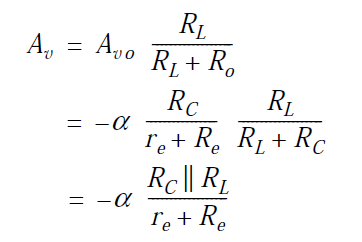
\includegraphics[width=\linewidth]{imgs/1}
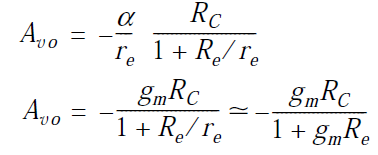
\includegraphics[width=\linewidth]{imgs/2}
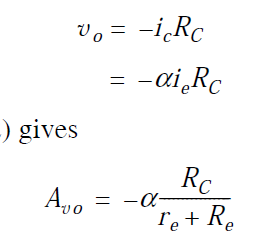
\includegraphics[width=\linewidth]{imgs/3}
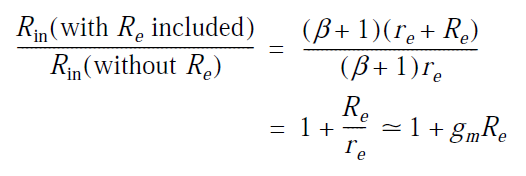
\includegraphics[width=\linewidth]{imgs/4}

\hrl

\textbf{Common base:}

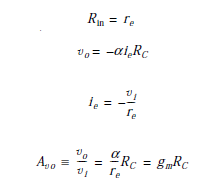
\includegraphics[width=\linewidth]{imgs/11}
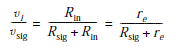
\includegraphics[width=\linewidth]{imgs/12}
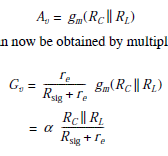
\includegraphics[width=\linewidth]{imgs/13}

\hrl 
\textbf{Common collector:}

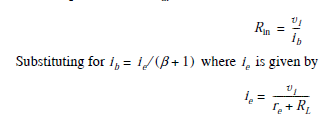
\includegraphics[width=\linewidth]{imgs/21}
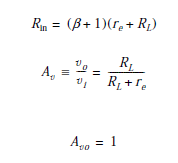
\includegraphics[width=\linewidth]{imgs/22}
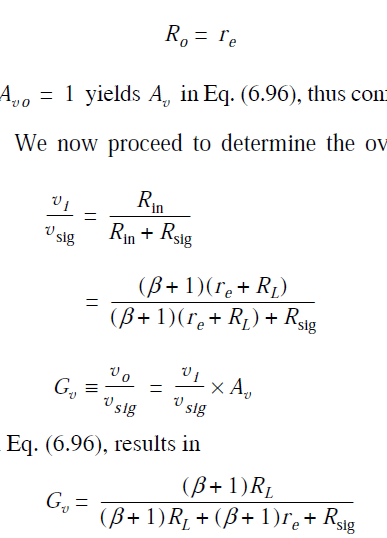
\includegraphics[width=\linewidth]{imgs/23}
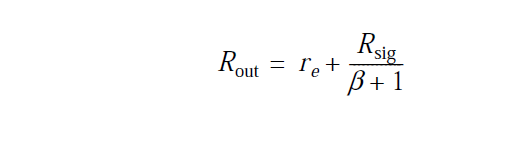
\includegraphics[width=\linewidth]{imgs/24}

\end{multicols}

\end{document}
